\section{目的與規格對照}
依講義 Lab 4（PDF 第 17--20 頁）比較三輸入 NAND 的擴散區幾何、接面寄生電容與固定電容近似。實驗步驟 1 要求 ACM=2/3 比較，步驟 2 要求各節點電容計算，步驟 3 要求以 $(C_{\max}+C_{\min})/2$ 代入並比較。

本次可完成明示 AD/AS/PD/PS 的幾何敏感度比較、接面電容數值抽取、節點電容加總與固定 C 模擬。由於所提供模型加密且缺少對應製程設計規則，本報告不宣稱已直接修改模型 ACM 選項或確認 foundry HDIF。這是有明確限制的電路模擬版本，並未進行 layout、DRC、LVS 或版圖寄生抽取。

\section{電路與手算幾何}
三個 PMOS 並聯拉高、三個 NMOS 串聯拉低；各 MOS 均使用 $W=1.8\,\mu$m、$L=0.25\,\mu$m。輸入 A 切換，B=C=1，外部負載 10 fF。另保留只寫 W/L 的模型預設分支作為參考。

採用教學幾何 $H=0.27\,\mu$m，僅作可重現的敏感度設定，不視為此模型的最小設計規則。對未共用的矩形擴散區，講義 ACM=2 方程為 $A=2HW$、$P=2(2H+W)$；得到 $A=0.972\,\mu$m$^2$、$P=4.68\,\mu$m。講義 ACM=3 的未共用端為 $A=2HW$、$P=4H+W=2.88\,\mu$m；共用端則為 $A=HW=0.486\,\mu$m$^2$、$P=2H=0.54\,\mu$m。A/B/C 的共用形式分別對應 GEO=2/3/1，數值直接寫入 instance 的面積及周長，不依賴不可見的模型選項。NRD=NRS=H/W=0.15。

接面電容的一般式可寫為
\[ C_j(V)=\frac{A C_{j0}}{(1+V/\Phi)^m}+\frac{P C_{jsw0}}{(1+V/\Phi_{sw})^{m_{sw}}}. \]
加密模型沒有提供可核對的全部係數，因此不捏造手算製程數值。改以關閉通道的 NMOS/PMOS 分別量測 drain 與 source，在 1 MHz 施加 1 V 小訊號並扣除同偏壓、零面積與零周長對照分支：$C_j=-\Delta\operatorname{Im}(I)/(2\pi f)$。反向偏壓採 0、0.25、0.5、0.75、1 V，保留實際偏壓相依性。

\section{模擬設定與量測定義}
本次使用獨立提供的 MOS 模型，電源為 1.0 V、溫度為 $27\,^{\circ}$C，並保留講義的電路拓樸及下列比較條件。1 V 是本次模擬設定，並非由公開模型文件確認的元件額定值；不能把講義舊製程的數值當成此次模型的驗收值。

模擬使用 HSPICE S-2021.09、RUNLVL=6。表格取自實際原生量測結果，圖形由實際列印數據重繪；每個變體都完整重設掃描參數及溫度，避免前一個變體的設定殘留。數值求解完成與量測成功，不等於已驗證製程可靠度。加密模型區塊的內部警告仍無法完整檢視。
輸入 0--1 V，PULSE 的上升與下降參數皆為 100 ps，週期 20 ns，暫態長度 40 ns、列印間距 2 ps。延遲採輸入／輸出 50\% 交越，輸出轉換時間採 10--90\%。

\section{模擬結果}
三個 netlist 共七個變體均完成求解，沒有錯誤或失敗量測。下表為幾何比較的延遲及轉換時間，單位 ps。

\begin{center}\small
\begin{tabular}{lllll}
\toprule
幾何 & $t_{pHL}$ & $t_{pLH}$ & $t_r$ & $t_f$ \\
\midrule
模型預設 & 70.30 & 127.58 & 165.68 & 92.29 \\
未共用 & 84.81 & 160.89 & 230.57 & 123.18 \\
共用 & 75.74 & 138.84 & 186.59 & 101.34 \\
\bottomrule
\end{tabular}
\end{center}
\begin{figure}[htbp]
\centering
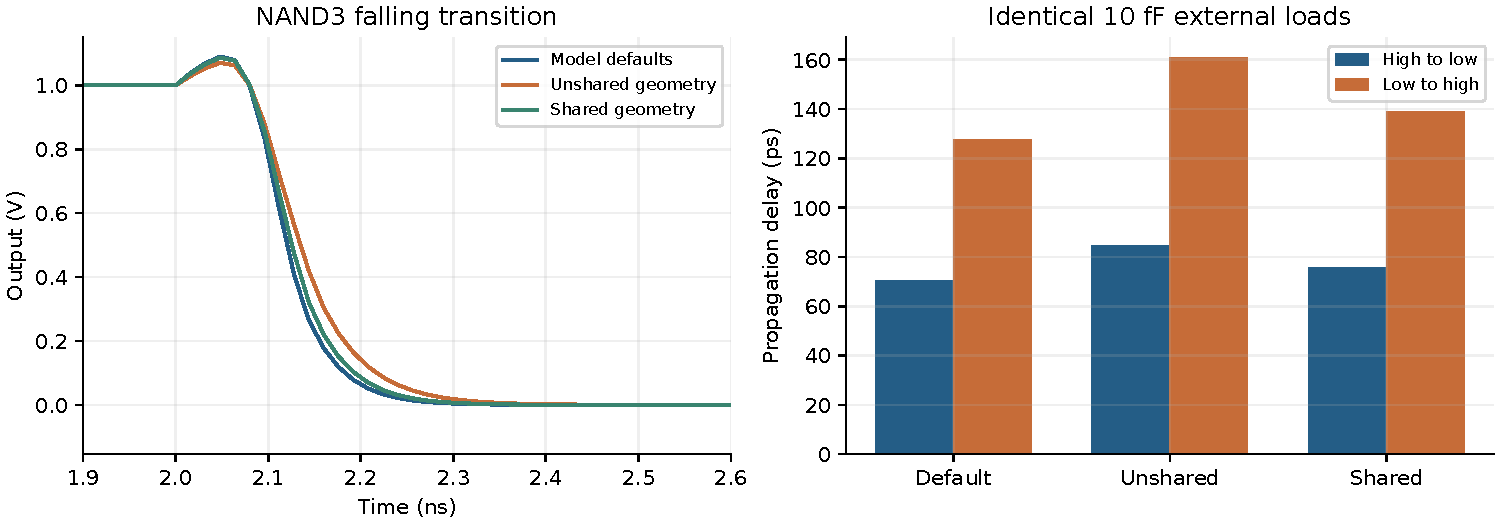
\includegraphics[width=\linewidth]{figures/diffusion_geometry.pdf}
\caption{明示幾何下的 NAND 延遲與實際下降波形。}
\end{figure}
\section{節點電容與固定 C 近似}
未共用幾何的輸出接面電容為 $3C_{p,d}+C_{n,d}$，內部 n1/n2 為相鄰 NMOS 的 source 與 drain 電容之和。共用幾何依各端的共享方式分別加總。各終端先取偏壓掃描的 $(C_{\max}+C_{\min})/2$，再組成節點電容；下表單位 fF。固定 C 分支把原本 AD/AS/PD/PS 設為零，再接入表中的電容，避免重複計算；內在通道電容、模型其他效應與外部 10 fF 負載仍保留。

\begin{center}\small
\begin{tabular}{lll}
\toprule
幾何模式 & Node & C (fF) \\
\midrule
2 & y & 8.6305 \\
2 & n1 & 4.1352 \\
2 & n2 & 4.1352 \\
3 & y & 3.3841 \\
3 & n1 & 0.5276 \\
3 & n2 & 0.5276 \\
\bottomrule
\end{tabular}
\end{center}
\begin{center}\small
\begin{tabular}{lll}
\toprule
模式 & $t_{pHL}$ dependent/fixed (ps) & $t_{pLH}$ dependent/fixed (ps) \\
\midrule
2 & 84.85 / 88.32 & 161.01 / 171.80 \\
3 & 75.75 / 78.30 & 139.00 / 145.06 \\
\bottomrule
\end{tabular}
\end{center}
\begin{figure}[htbp]
\centering
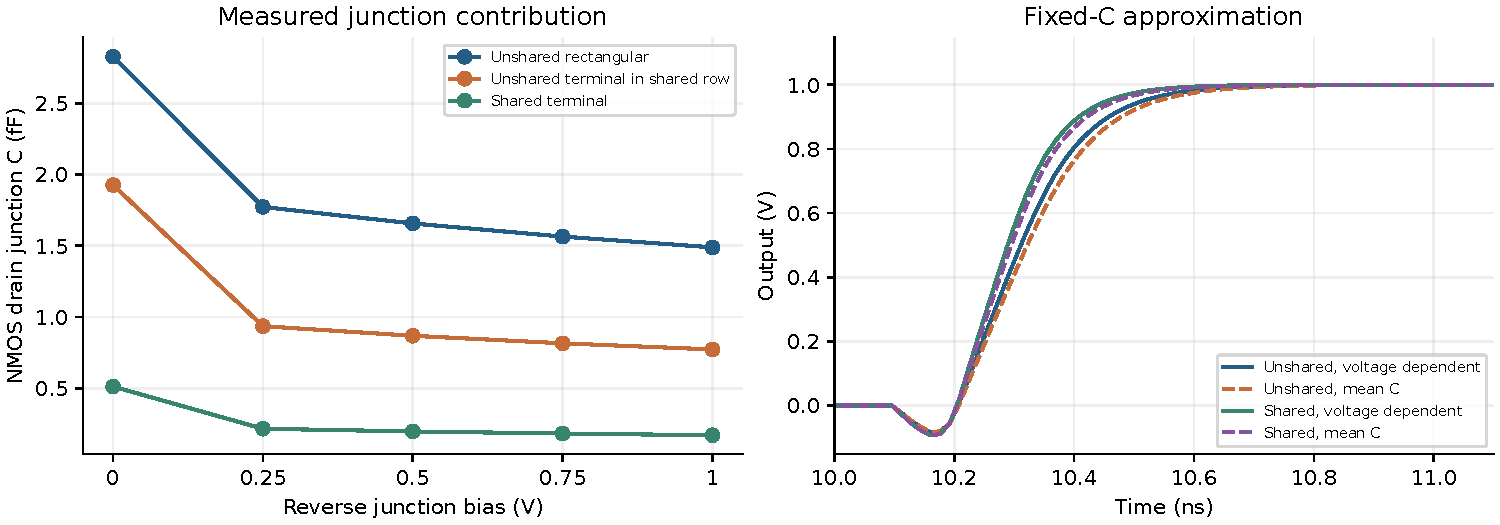
\includegraphics[width=\linewidth]{figures/junction_capacitance.pdf}
\caption{接面偏壓相依性，以及固定平均電容的上升波形比較。}
\end{figure}
\section{討論與限制}
共用擴散區減少面積及周長，因此本次的附加接面負載與延遲均降低。固定平均電容不能完整追蹤轉換過程中的偏壓變化：未共用分支的下降／上升延遲誤差為 4.09\%／6.70\%，共用分支為 3.36\%／4.36\%。所有固定 C 結果皆稍慢，不能把平均電容近似視為逐點等價。

本次驗證的是講義幾何方程及平均電容近似對電路的影響；literal ACM=2/3 模型開關、foundry HDIF 與完整係數手算仍未得到驗證。模型預設分支不應被稱為已知的 ACM=2。

\section{可重現檔案}
本實驗上傳下列 netlist；模型設定以註解標記保留，模型檔與其路徑均不隨報告上傳。執行前須在本機補入合法可用的模型設定。
\begin{itemize}
\item \texttt{01\_geometry.sp}
\item \texttt{02\_junction\_capacitance.sp}
\item \texttt{03\_constant\_capacitance.sp}
\end{itemize}
每一個變體的完整量測值位於本 lab 的 \texttt{results}，並附代表性波形 CSV、分析結果與規格對照清單。波形 CSV 最多保留 2501 個均勻取樣點；直接量測未降採樣。完整原始 listing 留在本機。

